\documentclass{article}
\usepackage{fullpage}
\usepackage{amsmath}
\usepackage{url}
\usepackage{graphicx}
\title{Fitting ODE solutions to noisy data by collapsing onto the manifold of solutions}
\author{Harry Braviner}

\date{\today}

\begin{document}
\maketitle

\section{Statement of the problem}

We have a collection of datapoints, $\left\{ \tilde{x}(t_i) \right\}$, and an ODE, $\mathcal{D}\left[ x; t \right] = 0$. We believe that the datapoints \emph{may be} noisy samples from \emph{some} solution to this ODE, but we do \emph{not} have a guess for the intial or bounday conditions. How can we evaluate the goodness-of-fit of this ODE (which we probably cannot solve analytically, and which we do not have initial conditions for) to these datapoints?

Let's simplify the problem space by making two big restrictions:
\begin{enumerate}
\item We only consider only one-dimensional second-order ODEs. i.e. the differential operator $\mathcal{D}\left[x ; t \right]$ has the form $\ddot{x}(t) - f\left(x(t), \dot{x}(t), t\right)$.
\item The datapoints, $\tilde{x}(t)$, are samples from an evenly-spaced discrete grid of times, $t_0, t_1, \dots, t_{N-1}$, where $t_i - t_{i-1} = h$. The samples themselves need not be evenly spaced: e.g. our dataset could consist of $\left\{\tilde{x}(t_0), \tilde{x}(t_1), \tilde{x}(t_2), \tilde{x}(t_{50})\right\}$. We also assume that we have at most one sample from any $t_i$. i.e. we never have multiple samples from the same time with different noise components.
\end{enumerate}

I am not concerned at this point about where $f$ comes from.
The motivation for everything in this document is that I would like to be able to modify PySR to search for such an $f$.
Doing so requires%
\footnote{It also requires modifying PySR to output functions of $t$, $x(t)$, and $\dot{x}(t)$, but I believe that is comparatively straightforward: have PySR treat $t$, $x(t)$ and $\dot{x}(t)$ as three independent variables.}
evaluating the goodness-of-fit of each $f$ to the data, and this work is intended to provide a method of doing so.

The essential idea I shall outline is this: We will approximate the (infinite dimensional) space of functions on $\left[t_{\mathrm{start}}, t_{\mathrm{end}} \right]$ by an $N$-dimensional discretization
$$
\left( \hat{x}(t_0), \hat{x}(t_1), \dots, \hat{x}(t_{N-1} \right)
$$
Within this $N$-dimensional space there is some subspace (the \emph{solution space}) that satisfies the ODE.%
\footnote{
And for a one-dimensional second-order ODE this subspace should generally be 2-dimensional.
}
\textbf{We shall collapse the $N$-dimensional discretization onto the solution space \emph{along the path minimizing the MSE of the data}.}
I shall be more precise about what this means in section \ref{sec:method}, after briefly reviewing other work and ideas.

\subsection{Previous work}

I haven't done a very comprehensive literature review, so I can't rule out that someone has done something similar to myself.
However, a little googling hasn't turned up anything identical.
I'll review here what I \emph{did} find, since a lot of this is quite interesting, might provide inspiration along different directions, and I want to at least have it written down for my own purposes.

In \cite{kronberger2019identification} the authors consider symbolic regression of first-order autonomous dynamical systems:
\begin{align}
\dot{x}_1(t) &= f_1\left(x_1, \dots, x_n\right) \nonumber \\
\dot{x}_2(t) &= f_2\left(x_1, \dots, x_n\right) \nonumber \\
 & \vdots \nonumber \\
\dot{x}_n(t) &= f_n\left(x_1, \dots, x_n\right) \nonumber \\
\end{align}
The candidate system, $\left( f_1, f_2, \dots, f_n\right)$, is the output of a genetic algorithm, although it does not appear to be PySR.
The authors use two methods of evaluating the goodness-of-fit of the ODE to the datapoints:
\begin{enumerate}
\item Using the approximate derivative values as a target, i.e.
$$
\mathrm{Loss}(f) = \sum_{i, j} \bigg(f_i\left( x_1(t_j), \dots, x_n(t_j) \right) - \big(x_i(t_{j+1}) - x_i(t_j)\big) \bigg)^2
$$
\item Integrating from the initial values $(x_1(t_0), ..., x_n(t_0))$ using a numerical ODE solver.
\end{enumerate}
The method of \cite{kronberger2019identification} does not appear to allow for noise in the measurements.
The results section shows the method being less successful on motion-captured data vs simulated data, and this supports my belief that this method does not tolerate measurement noise well.
They also assume that their datapoints are evenly spaced in time, although I'm not sure this is necessary. However, for method (1) to work, it is necessary for the spacing between the datapoints to be such that the numerical gradient is a good approximation to the true gradient.

\cite{bongard2007automated} also appears to integrate the candidate ODE from initial conditions that are assumed to be know.
The authors describe a system which not only evaluates candidate dynamical systems, but also suggests new experiments (i.e. initial conditions) that should best disambiguate between currently-strong candidates.
While this is a useful capability, and possibly the reason that the authors assume the initial conditions are known (because you set up the exeriment), it neglects the fact that in reality we never quite set up the system as we intend to.
The paper also assumes that the system is first order.

In \cite{iba2008inference} it is not clear how the authors obtain initial conditions, but I think that they simply take the same initial conditions used to generate the data and pass these, along with the candidate system, to the ODE integrator. Again, this paper condiders first order dynamical systems.

In \cite{d2023odeformer} the authors implement an end-to-end deep learning approach.
Input observations (i.e. $(x_1(t_i), \dots x_n(t_i), t_i)$) are embedded and then passed to a transformer, which outputs $(f_1, \dots, f_n)$ in the form of a string of symbols representing the tree form of the $f$s in prefix notation.
The model is trained on a randomly generated synthetic dataset.
This has the advantage that the target string is known (because it was generated at random), and the input data (the samples) are generated by numerical integration of the $f$.
The authors do consider noisy data and non-uniform spacing ('subsampling').
This paper completely sidesteps the issue of how to evaluate the goodness-of-fit without the underlying initial conditions: we do not have to repeatedly evaluate the goodness-of-fit of $f$s, because we only have a single candidate, the output of the transformer.
Unlike PySR, this method does not produce a Pareto front.

The issue \cite{pysrissue568} on the PySR github repo suggests that, at least as of March 2024, the accepted method for performing SR for an ODE was haveing PySR generate both the ODE and the initial conditions.
This has two issues.
First, the additional time taken to search for initial conditions (and all of the problems I will discuss in the next section regarding sweep-and-shoot approaches).
Secondly, outputting an ODE and an intial condition allows us to test only a single dataset.
We might have multiple timeseries that we believe obey the same ODE with different initial conditions.

In issue \cite{pysrissue732} Miles refers someone looking to do SR on ODEs to \cite{pysrchangenotev1.3.0}, which suggests performing integration of a function by generating data points for the integrand, and then performing SR on candidate expressions for the integral.
Could this method be applied to an ODE (by replacing the dataset generated from the integrand in \cite{pysrchangenotev1.3.0} by the timeseries)?
One limitation of doing so is that we are now searching over the expression for the \emph{solution to} the ODE.
Many physical systems have a simple expression in terms of ODEs, but no closed form solution to that ODE.

\subsection{Alternative methods}

In this section I'm going to outline some alternative methods that seem attractive.

\subsubsection{Extracting $\dot{x}(t)$ from the data}
\label{sec:alternate_extracting_xdot}

Several of the papers described above evaluate $f$ directly as the degree of disagreement between $f(x(t))$ and $\dot{x}(t)$ as approximated by forward differences from the data samples.
Even if the samples have zero noise, the descretization of the time-sampling can cause considerable error in the approximation (see figure \ref{fig:deriv_from_samples}), and the addition of noise makes the error much worse (see figure \ref{fig:deriv_from_noisy_samples}).
The method I outline in the note should be able to handle much sparser and noisier samples.

\begin{figure}
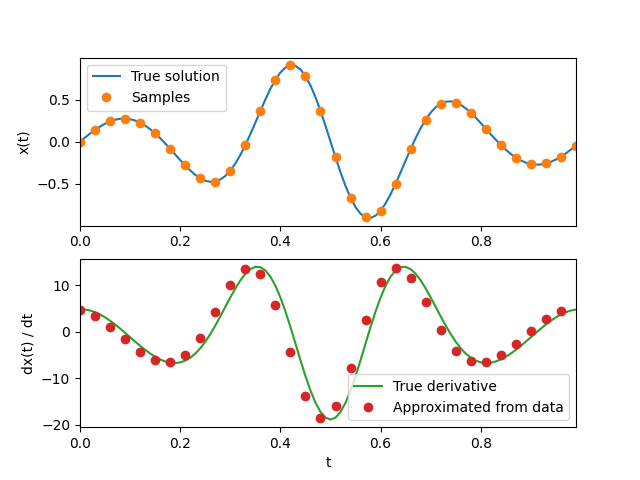
\includegraphics{images/alternative_methods/deriv_from_samples.png}
\centering
\caption{Forward numerical derivative, $\left(x(t_{i+1}) - x(t_i)\right)/\left(t_{i+1} - t_i\right)$ from sampled data. There is some error, with the derivative being shifted left, even though the points are densely spaced.}
\label{fig:deriv_from_samples}
\end{figure}

\begin{figure}
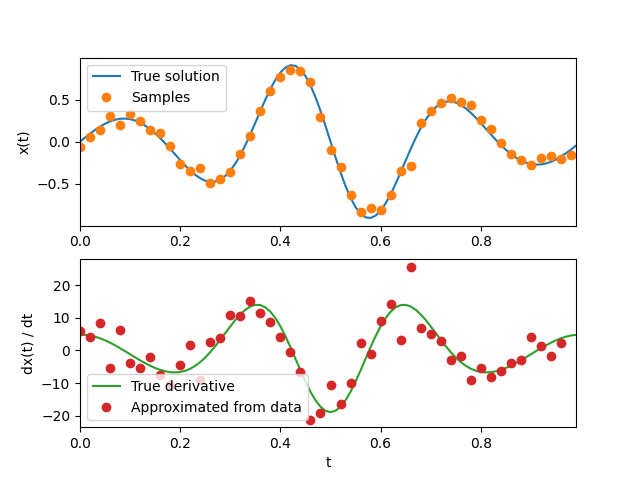
\includegraphics{images/alternative_methods/deriv_from_noisy_samples.png}
\centering
\caption{Forward numerical derivative, $\left(x(t_{i+1}) - x(t_i)\right)/\left(t_{i+1} - t_i\right)$ from sampled data with Gaussian noise with $\sigma = 0.05$. The error is considerably worse than in figure \ref{fig:deriv_from_samples}.}
\label{fig:deriv_from_noisy_samples}
\end{figure}

\subsection{Smoothing the data with a kernel}
\label{sec:smoothing}

Smoothing the datapoints with some kernel function (e.g. a rolling average window) would go some way toward addressing the issue of noise in the dataset.
PySR supports something similar to this feature via the \texttt{denoise} option, which first fits a Gaussian process to the data.
This could be modified to also output the gradient of the fitted process.
One downside of this method is that it requires the choice of hyperparameters for the kernel of the Gaussian process (I don't think PySR exposes these choices to the end user, and I'm not sure if it has some clever way to pick them).

A second, more subtle problem exists with both this method and that of section \ref{sec:alternate_extracting_xdot}. If the data sampling is sufficiently irregular, checking that the candidate ODE is obeyed locally is \emph{not} the same as verifying that it is obeyed globally.
This is illustrated in figure \ref{fig:gp_fitting}.
A Gaussian process is fitted to two clusters of sampled datapoints.
Comparing the second derivative of the Gaussian process to the right hand side of $\ddot{x}(t) = -(2\pi10)^2 x(t)$ gives excellent agreement, and we might conclude that this data comes from a 10Hz harmonic oscillator.
But it does not.
In the upper plot of figure \ref{fig:gp_fitting} we also show two solutions for a 10Hz harmonic oscillator, with different initial conditions.
It is clear that one cluster of sampled datapoints fits one set of initial conditions, and the other cluster fits the other set.
But the whole cluster as a single timeseries does not fit this candidate ODE for any set of initial condtions.

\begin{figure}
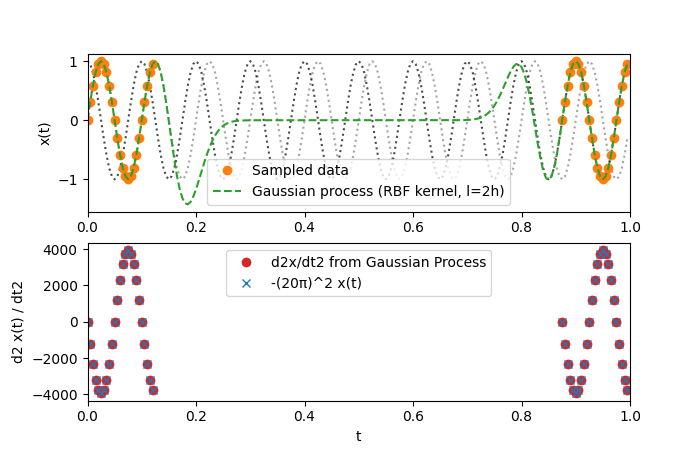
\includegraphics{images/alternative_methods/gp_fitting.png}
\centering
\caption{A Gaussian process is fitted through sampled datapoints (top plot), and the second derivative of this process is compared to the right-hand side of the candidate equation $\ddot{x}(t) = -(2\pi10)^2 x(t)$ (bottom plot) where excellent agreement is seen (the relative error is a few parts-per-thousand).
However, the two clusters of datapoints come from solutions of this ODE that have different initial conditions, being $90^{\circ}$ out of phase (dotted lines on the top plot).
}
\label{fig:gp_fitting}
\end{figure}

We should note that this is not an artifact of the Gaussian process.
This issue would arise even if we had access to measured values of $\ddot{x}(t)$ at the sample points.

One could object that I have cheated by only evaluating the Gaussian process and its second derivative at the sampled points.
Should we have compared $\hat{x}$ from the Gaussian process to its second derivative over the whole range?
I believe not.
Doing so here would show serious divergence from the ODE $\ddot{x} = -(2\pi10)^2 x$ in the middle of the domain.
\emph{But it would also do so if the datapoints were drawn from the same solution.}
We would mark \emph{any} candidate ODE as a poor fit to data with large gaps in its time-sampling.
The Gaussian process only helps us \emph{interpolate}; it is not reasonable to expect it to also \emph{extrapolate}.

\subsection{Sweep-and-shoot methods}
\label{sec:sweep_and_shoot}

If we knew the intial conditions for our dataset, we could integrate from the earliest point using a numerical ODE solver and compare the numerically integrated solution, $\hat{x}(t)$, to the sampled solution $\tilde{x}(t)$, at every later sampling time.
This works well if the initial conditions are known with zero noise.
In practice, noise may be present, and this method privileges the first point (by treating it as noiseless) in a way that we would probably prefer to avoid.
In the case of second order ODEs, we need to either have direct measurement of $\tilde{\dot{x}}$ or use the first two points to approximate it.

In the absence of noiseless initial conditions, we can `sweep' over plausible values and integrate the ODE forward in time (`shoot') for each set of initial conditions.
The noisy values for the first $x$ and $\dot{x}$ could be used as a point around which to centre the sweep.

This approach is viable for a low dimensional problem, but will become exponentially expensive as the number of dimensions increases.
If we choose to sweep over $10$ values for each inital condition for a 3 dimensional second order ODE ($x$, $\dot{x}$, $y$, $\dot{y}$, $z$, $\dot{z}$) we would have $10^6$ combinations to try.

Even in low-dimensional problem, sweep-and-shoot can struggle to evaluate whether the ODE is a good fit to the data. Consider the system
$$
\ddot{x}(t) = - x(t)^3 + a^2 x(t) - \nu \dot{x}(t)
$$
This system is a double-well potential with stable fixed points at $x = \pm a$ (with small oscillation frequencies of $\sqrt{2 a^2 - \nu^2/4}$) and an unstable fixed point at $x=0$ (with $x(t) \approx A_0 \exp(a (t - t_0)$ around this point).

\begin{figure}
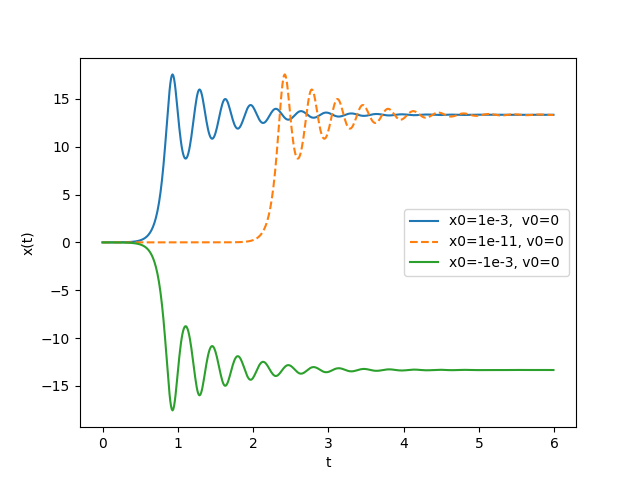
\includegraphics{images/alternative_methods/double_well.png}
\centering
\caption{
Three (numerically integrated) solutions to $\ddot{x}(t) = -x(t)^3 + a^2 x(t) - \nu \dot{x}(t)$ for $a = 6\pi / \sqrt{2}$ and $\nu = 3$.
Note that the initial conditions have identical velocities and differ very small values of the $x$ coordinate.
}
\label{fig:double_well}
\end{figure}

Figure \ref{fig:double_well} shows three solutions to this system, for very similar initial conditions.
Suppose that our experiment had evolved along the dashed, orange curve ($x_0 = 10^{-11}$, $v_0 = 0$), and we had samples from it.
If we were performing a sweep-and-shoot search, we might well have integrated from $x_0 = 10^{-3}$, produced the blue curve, and measured this to have high MSE relative to our data.
We would then step our initial condition to our next point, $x_0 = -10^{-3}$, and produce the green curve, having an even higher MSE.
We would reject the candidate ODE, despite it being completely correct!

One might object to this, saying that clearly the sweep should be performed in log-space since we are so close to $x=0$.
This is true, but we know this because we are applying our intelligence and knowledge of the underlying ODE.
The location of an unstable fixed point will not always be at zero.
To first locate the fixed points of the candidate ODE and treat them as special in a sweep-and-shoot procedure would be considerable additional algorithmic complexity.
(In fact, taking the initiative to do so might be a good desideratum of an AI physicist!)

\subsection{Relaxation methods}

The method I describe below will look a bit like a relaxation method (see \cite{wikipediaRelaxationMethod}), and one might wonder if some variation of this could be used to achieve faster convergence.
This might be the case, but if so I haven't yet figured out how.

The relaxation method seems to require fixed, known end-points.
i.e. it requires boundary conditions.
We could take the earliest and last sampled datapoints, and use these as boundary conditions.
However, that would (just like shooting from the first point) elevate these points in significance by assuming that they have no measurement noise.
We would also have a version of the problem indicated in figure \ref{fig:double_well}: the blue and orange curves have extremely similar boundary conditions if $t_{\mathrm{start}}$ is sufficiently early, $t_{\mathrm{end}}$ significantly late.

\section{The Collapse Method}
\label{sec:method}

There are two different ways to think of the problem of how well an ODE fits a sampled dataset. Every paper I have been able to find on this subject implicitly does one or the other, but none of them seem to discuss the fact that the other viewpoint exists, or even explicitly acknowledge their choice.
\begin{enumerate}
\item Fit the data exactly and measure the extent to which the ODE is violated. e.g. $L_{\mathrm{ODE}} = \sum_i \left( \tilde{\ddot{x}}(t_i) - f(\tilde{x}(t_i), \tilde{\dot{x}}(t_i), t_i)\right)^2$.
This is the approch of most papers that approximate the derivative by finite differences between datapoints (though, as we discussed in section \ref{sec:smoothing}, you could fit a smoothing function instead).
\item Insist on the ODE being obeyed, and measure the error of the data relative to the solution, e.g. $L_{\mathrm{data}} = \sum_i \left( \hat{x}(t_i) - \tilde{x}(t_i) \right)^2$.
This is the approach of papers where the candidate ODE is numerically integrated. It requires some way of obtaining initial conditions. 
\end{enumerate}

\begin{figure}
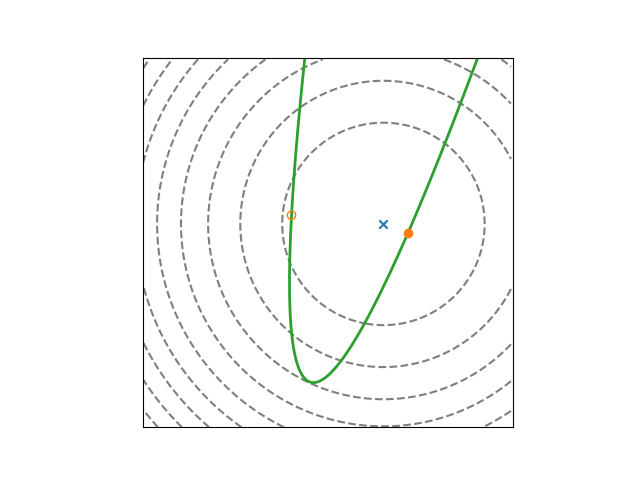
\includegraphics{images/method/disc_space_viz.png}
\centering
\caption{
Schematic representation of discretized solution space.
Gray dashed curves are contours lines of the data loss, $L_{\mathrm{data}}$.
The solid blue dot shows the (global and only) minimum of $L_{\mathrm{data}}$.
The heavy green curve is the solution space, and the orange circles denote the minima of $L_{\mathrm{data}}$ restricted to the solution space (the hollow circle is a local minimum, the solid circle a global minimum).
}
\label{fig:disc_space_viz}
\end{figure}

The second approach (satisfying the ODE and evaluating the error in fitting the data) feels better-defined.
It is unclear that the extent-of-violation of an ODE is well-captured by the squared-error of the difference between the two sides of the equation.

However, there are pitfalls with this.
It may be difficult to find initial conditions, as discussed in section \ref{sec:sweep_and_shoot}.
Even if we were able to backpropogate through the ODE solver to compute the gradient of $L_{\mathrm{data}}$ with respect to our initial conditions, the loss function restricted to the solution-space may not be convex.
This is illustrated in figure \ref{fig:disc_space_viz}: if we start near the local minimum of the solution space, we will never find the global minimum by any method of small steps.

What I have therefore implemented is approach (1) followed by approach (2).

We begin by discretizing the space of functions on $[t_0, t_{N-1}]$ as a vector
$$
\left( \hat{x}(t_0), \hat{x}(t_1), \dots, \hat{x}(t_{N-1}) \right)
$$
which for notational convenience I will call
$$
\left( \hat{x}_0, \hat{x}_1, \dots, \hat{x}_{N-1} \right)
$$
from here on.
We require that these grid-points be evenly spaced, and denote the step-size as $h = t_i - t_{i-1}$.

Remember that we have measurements from only some of these times.
Let $\mathcal{I}$ denote the set of indices such that we have a measurement $\tilde{x}(t_i)$ at time $i$.
Again, for notational convenience I will call these measurements $\tilde{x}_i$ from here on.
These measurements may contain noise.

We now define two loss functions:%
\footnote{
We could instead use the backward derivative, $\hat{\dot{x}}(t_i) = h^{-1} \left( \hat{x}(t_{i}) -  \hat{x}(t_{i-1})\right)$. I do not think this should make a difference, but I have added an option to do so in my code.
}
\begin{align}
\label{eq:Ldata}
L_{\mathrm{data}} &= \frac{1}{2} \frac{1}{\left| \mathcal{I} \right|} \sum_{i \in \mathcal{I}} \left( \hat{x}_i - \tilde{x}_i \right)^2 \\
\label{eq:Lode}
L_{\mathrm{ODE}} &= \frac{1}{2} h \sum_{i=1}^{N-2} \left( \hat{\ddot{x}}_i - f\left( \hat{x}_i, \hat{\dot{x}}_i, t_i \right) \right)^2 \\
\mathrm{where} \, & \, \hat{\ddot{x}}_i = h^{-2} \left( \hat{x}_{i-1} - 2\hat{x}_i + \hat{x}_{i+1} \right) \\
\mathrm{and} \, & \, \hat{\dot{x}}_i = h^{-1} \left( \hat{x}_{i+1} - \hat{x}_i \right)
\end{align}

Note the range of the sum in \eqref{eq:Lode}: we could not extend this to $i=0$ or $N-1$, since we would not have the points $\hat{x}_{-1}$ and $\hat{x}_N$ needed to define the second derivative.
But this should not concern us.
Imagine that our task was to set $L_{\mathrm{ODE}}$ to zero.
Each term must vanish individually, so the sum gives us $N-2$ equations in $N$ unknowns ($\hat{x}_0, \dots, \hat{x}_{N-1}$).
For most choices of $f$ we will not be able to solve these equations, but for $N-2$ equations in $N$ unknowns we expect that, if a solution space exists, it will be 2 dimensional.
And that is exactly what we expect for a second-order ODE.

We begin by minimizing $L_{\mathrm{data}}$ (an easy task, since this is a convex loss function with constant curvature), and then minimize $L_\mathrm{ODE}$.
In practice we do this by gradient descent, minimizing
$$
L_{\mathrm{total}} = (1 - W_{\mathrm{ODE}}) L_{\mathrm{data}} + W_{\mathrm{ODE}} L_{\mathrm{ODE}}
$$
and varying $W_{\mathrm{ODE}}$ from close to zero at the start training to close to one at the end of training.
Schematically, we first proceed to the blue cross (exactly fitting the data) in figure \ref{fig:disc_space_viz}, and then to the green curve (the solution space).
Due to going via the blue cross, we should arrive at the solid yellow circle (the global minimum of $L_{\mathrm{data}}$ on the solution space).

Since we are collapsing the vector onto the lower-dimensional solution space, I will refer to this method as \emph{the collapser}.

\subsection{Reducing the stiffness of the optimization problem}

After implementing this method I initially tried it on an extremely simple system
$$
\ddot{x}(t) = F
$$
for constant $F$.

The method described above struggled to produce a good fit to this system at all.
Simple gradient descent required incredibly small step sizes ($\sim 10^{-7}$) otherwise NaNs would appear in the solution.
Reducing the step size sufficiently that this no longer occurred resulted in solutions that satisfied the ODE, but were a poor fit to the data, even with zero noise.

At first I suspected the system was getting stuck in a local optimum, but this isn't possible - with constant acceleration the discretized system is convex.
A little further investigation revealed that the problem was likely due to the condition number%
\footnote{
The Hessian of $L_{\mathrm{ODE}}$ actually has two zero eigenvalues (corresponding to the tangent space of the solution space). When I say `condition number' I mean the ratio of the largest eigenvalue to the smallest non-zero eigenvalue.
}
 of the Hessian of $L_{\mathrm{ODE}}$ being very large.%
\footnote{
During my time at Layer 6 I used to ask prospective colleagues an interview question about the maximum learning rate they could use on a loss function $L(x, y) = \frac{1}{2} \left( a x^2 + b y^2 \right)$ for $ a \gg b$.
I suspect that me spending several hours debugging what amounts to a somewhat obfuscated version of the same problem is down to karma.
}

Since this simple version of the problem (constant acceleration) is the optimization of a quadratic function, I switched to \texttt{LBFGS}, an approximate quadratic optimizer provided by PyTorch that does not require explicitly computing second order derivative.
This partially solved the problem, in that it worked well for small numbers of grid points (10), but still worked very poorly on moderately sized grids (100 points).
In the latter case the ODE would typically be satified, but the solution would visually be a long way from the sample points.

If we directly compute the Hessian of $L_{\mathrm{ODE}}$ for this problem, we find
$$
\left[\frac{\partial^2 (h^3 L_{\mathrm{ODE}})}{\partial \hat{x}_i \partial \hat{x}_j} \right] = \begin{pmatrix}
1 & -2 & 1 & 0 & 0 & 0 & 0 & \cdots & 0 \\
-2 & 5 & -4 & 1 & 0 & 0 & 0 & \cdots & 0 \\
1 & -4 & 6 & -4 & 1 & 0 & 0 & \cdots & 0 \\
0 & 1 & -4 & 6 & -4 & 1 & 0 & \cdots & 0 \\
\vdots & \vdots & \vdots & \vdots & \vdots & \vdots & \vdots & \vdots & \vdots \\
0 & \cdots & 0 & 1 & -4 & 6 & -4 & 1 & 0 \\
0 & \cdots & 0 & 0 & 1 & -4 & 6 & -4 & 1 \\
0 & \cdots & 0 & 0 & 0 & 1 & -4 & 5 & -2 \\
0 & \cdots & 0 & 0 & 0 & 0 & 1 & -2 & 1 \\
\end{pmatrix}
$$

For 10 dimensions, this matrix has a condition number of
$$
\frac{\lambda_{\mathrm{max}}}{\lambda_{\mathrm{min}, \ne 0}} \approx \frac{7.55}{0.0253} \approx 299 \,.
$$
For 100 dimensions, the condition number is
$$
\frac{\lambda_{\mathrm{max}}}{\lambda_{\mathrm{min}, \ne 0}} \approx \frac{8.00}{2.50\times 10^{-6}} \approx 3.2 \times 10^6 \,.
$$

At this point I decided to try switching coordinates, defining
\begin{align}
\label{eq:zdef}
z_0 & = x_0 \nonumber \\
z_i & = x_i - x_{i-1} \, \mathrm{for} \, i \ge 1 
\end{align}
i.e. we work in gradient space, rather than position space.

In these coordinates the loss becomes 
$$
L_{\mathrm{ODE}} = \frac{1}{2} h \sum_{i=1}^{N-2} \left( h^{-2}(z_{i+1} - z_i) - F \right)^2 
$$
and the Hessian becomes
$$
\left[\frac{\partial^2 (h^3 L_{\mathrm{ODE}})}{\partial z_i \partial z_j} \right] = \begin{pmatrix}
0 & 0 & 0 & 0 & 0 & \cdots & 0 \\
0 & 1 & -1 & 0 & 0 & \cdots & 0 \\
0 & -1 & 2 & -1 & 0 & \cdots & 0 \\
0 & 0 & -1 & 2 & -1 & \cdots & 0 \\
\vdots & \vdots & \vdots & \vdots & \vdots & \vdots & \vdots \\
0 & \cdots & -1 & 2 & -1 & 0 & 0 \\
0 & \cdots & 0 & -1 & 2 & -1 & 0 \\
0 & \cdots & 0 & 0 & -1 & 2 & -1 \\
0 & \cdots & 0 & 0 & 0 & -1 & 1 \\
\end{pmatrix}
$$

This is considerably more benign. For 100 dimensions, the condition number of the Hessian with respect to the $z$ coordinates is
$$
\frac{\lambda_{\mathrm{max}}}{\lambda_{\mathrm{min}, \ne 0}} \approx 4.0 \times 10^3 \,.
$$
In figure \ref{fig:condition_numbers} we can see that the condition number with this transformation does continue to increase with the number of dimensions (i.e. with finer discretization of the time domain), but is clearly less stiff than the untransformed problem.

\begin{figure}
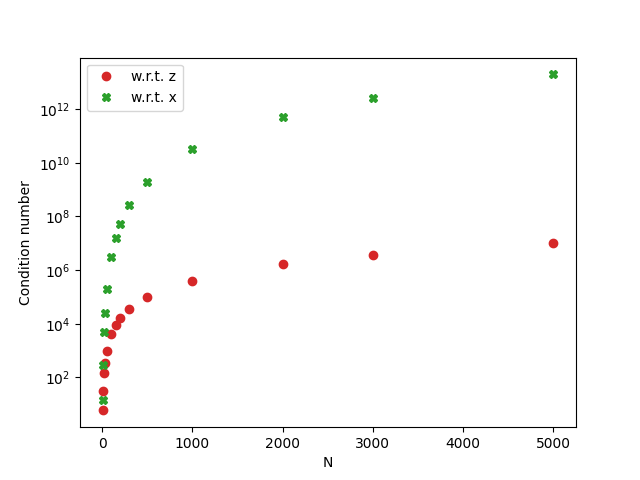
\includegraphics{images/method/condition_numbers.png}
\centering
\caption{
Condition number, $\lambda_{\mathrm{max}} / \lambda_{\mathrm{min}, \ne 0}$, for the Hessian of $L_{\mathrm{ODE}}$ with respect to the original variables, $\hat{x}_i$, and the $z_i$ defined by \eqref{eq:zdef}.
}
\label{fig:condition_numbers}
\end{figure}

In these coordinates, with a grid size of $N=100$, the optimization process appears to work.
I have not tested larger grid sizes yet.
One question that I do not have an answer to is whether there is a better coordinate transformation that could be applied.
My implementation uses the transformation \eqref{eq:zdef} by default, but does allow for any other linear transformation to be specified.

\section{Qualitative results}
\label{sec:qual_results}

Does this method (plus the coordinate transformation) actually produce discretizations that both satisfy the ODE and fit the data?

To test this, we generate some data from an underlying ODE%
\footnote{
Either using the analytic solution, or the ODE solver from SciPy.
}
and sample a few points from this curve, and add noise.
We pass these noisy points, and the ODE (but \emph{not} the intial conditions) to our method.
We show in figures \ref{fig:fit_const_acc}, \ref{fig:fit_sho}, \ref{fig:fit_damped_sho} and \ref{fig:fit_qd_osc} that it does indeed produce good fits to the underlying curves.
The results in figure \ref{fig:fit_qd_osc} are particularly gratifying, since this ODE does not have an analytic solution.

\begin{figure}
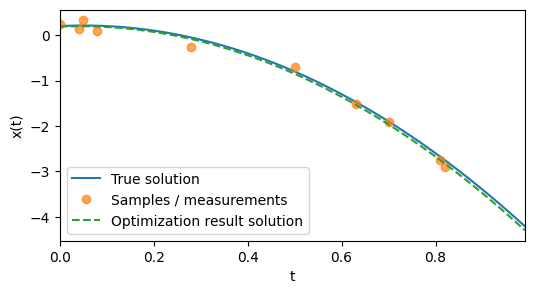
\includegraphics{images/results/fit_const_acc.png}
\centering
\caption{
Solution to the ODE $\ddot{x}(t) = -10$ with $x{0} = 0.2$ and $\dot{x}(0) = 0.5$ (blue curve), and a small number of samples (orange dots) plus Gaussian noise with $\sigma = 0.1$.
The output of the collapser method is shown as the dashed green curve.
The collapser has no access to the initial conditions that were used to generate the blue curve.
}
\label{fig:fit_const_acc}
\end{figure}

\begin{figure}
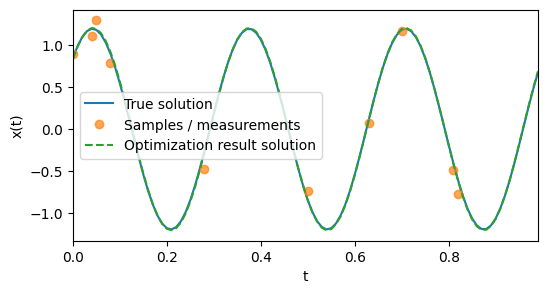
\includegraphics{images/results/fit_sho.png}
\centering
\caption{
Solution to the ODE $\ddot{x}(t) = - (6\pi)^2 x(t)$ with initial amplitude 1.2 and phase $pi/4$ (blue curve), and a small number of samples (orange dots) plus Gaussian noise with $\sigma = 0.1$.
The output of the collapser method is shown as the dashed green curve.
The collapser has no access to the initial conditions that were used to generate the blue curve.
}
\label{fig:fit_sho}
\end{figure}

\begin{figure}
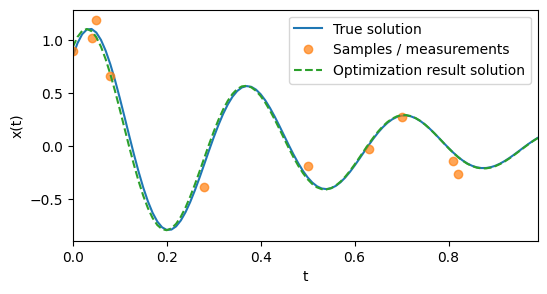
\includegraphics{images/results/fit_damped_sho.png}
\centering
\caption{
Solution to the ODE $\ddot{x}(t) = - (6\pi)^2 x(t) - 4 \dot{x}(t)$ with initial amplitude 1.2 and phase $pi/4$ (blue curve), and a small number of samples (orange dots) plus Gaussian noise with $\sigma = 0.1$.
The output of the collapser method is shown as the dashed green curve.
The collapser has no access to the initial conditions that were used to generate the blue curve.
}
\label{fig:fit_damped_sho}
\end{figure}

\begin{figure}
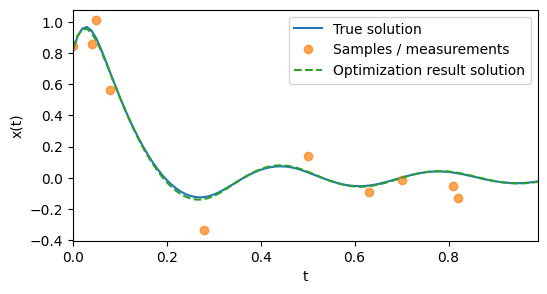
\includegraphics{images/results/fit_qd_osc.png}
\centering
\caption{
Solution to the ODE $\ddot{x}(t) = - (6\pi)^2 x(t) - 4 \dot{x}(t) \left| \dot{x}(t) \right|$ with $x(0) = 0.8$ and $\dot{x}(0) = 15$ (blue curve), and a small number of samples (orange dots) plus Gaussian noise with $\sigma = 0.1$.
The output of the collapser method is shown as the dashed green curve.
The collapser has no access to the initial conditions that were used to generate the blue curve.
}
\label{fig:fit_qd_osc}
\end{figure}

While these results are gratifying, remember that they are a necessary condition, but not a sufficient one, for this method to be useful to our purposes.
We want to evaluate the goodness-of-fit of the ODE to the data.
If we pass the \emph{wrong} ODE to the collapser (i.e. one that differs from the ODE used to generate the data), we want to collapser to prefer satisfying the ODE over matching the data.
In figure \ref{fig:badfit_qd_osc_sho} we demonstrate this.
We generate data from the same equation (a harmonic oscillator plus quadratic drag) as in figure \ref{fig:fit_qd_osc}, but give a different ODE to the collapser.
The collapser clearly outputs a solution to the simple harmonic oscillator equation, fitted to the data as best it can.
The difference shows up quantatively too: in figure \ref{fig:fit_qd_osc} $L_{\mathrm{data}} = 5.9 \times 10^{-3}$, and in figure \ref{fig:badfit_qd_osc_sho} $L_{\mathrm{data}} = 5.3 \times 10^{-2}$.
This is promising, as it suggests that this method can reject ODEs that are a poor fit to the data.

\begin{figure}
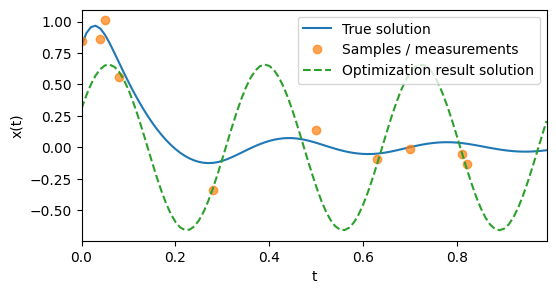
\includegraphics{images/results/badfit_qd_osc_sho.png}
\centering
\caption{
The data generation here is the same as in figure \ref{fig:fit_qd_osc}.
However, the collapser has been passed the ODE $\ddot{x}(t) = - (6\pi)^2 x(t)$.
This differs from the ODE used to generate the data, as the quadratic drag term is absent.
The output of the collapser method is shown as the dashed green curve, and clearly appears to be a simple harmonic, at the expense of fitting the data.
}
\label{fig:badfit_qd_osc_sho}
\end{figure}

All of the above results were generated using the notebook \texttt{demo\_notebooks/demo\_use\_of\_libraries.ipynb}.

\subsection{Large gaps in timeseries}

Recall that in section \ref{sec:smoothing} we construced an example (see figure \ref{fig:gp_fitting}) in which it was possible to fit the data well while satisfying the ODE locally, but not globally.
Will our collapser method handle this correctly, or will it build up small violations of the ODE in the region that is far from any sampled datapoint?
In figure \ref{fig:mismatched_oscillators} we run this experiment (see notebook \texttt{demo\_notebooks/mismatched\_oscillators.ipynb} to reproduce this) and find that the collapser behaves as desired: it enforces the ODE, at the cost of fitting the data.
In particular, it does not allow any form of `phase drift' in the gap between observations.

\begin{figure}
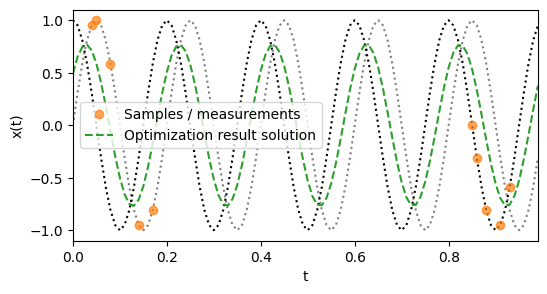
\includegraphics{images/results/mismatched_oscillators.png}
\centering
\caption{
We generate two sets of timeseries from oscilators of the same frequency, but $90^{\circ}$ out of phase.
We treat these as a single series, with the observations from one sampled at early times and the other at late times.
For this combined series, the ODE $\ddot{x}(t) = - \omega^2 x(t)$ should not fit the data.
We see that the collapser does indeed correctly enforce the ODE, and does not fit the data well.
}
\label{fig:mismatched_oscillators}
\end{figure}

\subsection{Unstable fixed points}

In figure \ref{fig:double_well} we showed 3 (numerically integrated) solutions for the ODE
$$
\ddot{x}(t) = - x(t)^3 + (6\pi/\sqrt{2})^2 x(t) - 3 \dot{x}(t)
$$
and claimed that it would be very hard for sweep-and-shoot method to discover appropriate initial conditions, and that such a method would falsely reject this ODE as a inconsistent with the data.
Can the collapser method find these solutions?

It can, but modifications needed to be made.
Using settings that produced the results of section \ref{sec:qual_results}, the collapser produced three curves that appeared to obey the ODE, but were very poor fits to that data.
Many of them `fell' into the opposite well compared to their sampled data.
Inspecting the evolution of $L_{\mathrm{data}}$ and $L_{\mathrm{ODE}}$ over the course of the optimization showed that $L_{\mathrm{data}}$ did not reach zero, even during the early stages of optimization where $W_{\mathrm{ODE}} = 10^{-2}$.
We should in fact be able to fit the data exactly if we ignore the requirement to satisfy the ODE.
So I first modified the code to initialize the discretized solution to a linear interpolation between the data points.

Initializing the discretized solution in this manner produced a good result on one of the three timeseries, but the other two still fit the data extremely poorly by falling into the wrong well.
Again inspecting the evolution of $L_{\mathrm{data}}$ and $L_{\mathrm{ODE}}$ showed that $L_{\mathrm{data}}$ spiked upwards to an extreme value at the start of the optimization, before decreasing somewhat.
This occurred even during the early `warmup' period when $W_{\mathrm{ODE}} = 10^{-2}$.
By decreasing $W_{\mathrm{ODE}}$ to $10^{-4}$ I was able to obtain the fits shown in figure \ref{fig:double_well_collapser}.

The results of figure \ref{fig:double_well_collapser} do show good fits.
The purple solution has been found almost exactly, and the blue has found a solution that matches the data very closely, even though it does not match the underlying solution.
The red solution is clearly a little lacking, but still appear good.
In each case the behaviour is qualitatively correct.

However, I believe this should be regarded as only a partial success for the collapser.
Manual intervention was required to obtain these solution.
Nor is the change I made here completely superior: I tried re-running the experiment of figure \ref{fig:fit_qd_osc} with these changes.
Initializing the discretization by interpolation still resulted in an excellent fit, but changing $W_{\mathrm{ODE}}$ to $10^{-4}$ for the warmup period caused the optimization to fail, producing NaNs.

More development is needed to make the optimizer widely useable, and I discuss this in section \ref{sec:numerical_stability}.

\begin{figure}
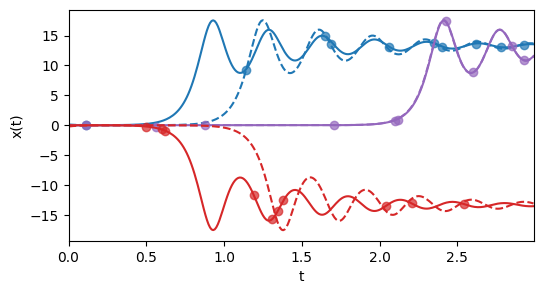
\includegraphics{images/results/double_well_collapser.png}
\centering
\caption{
The solid curves show three (numerically integrated) solutions to $\ddot{x}(t) = -x(t)^3 + a^2 x(t) - \nu \dot{x}(t)$ for $a = 6\pi / \sqrt{2}$ and $\nu = 3$.
The circles of the same colour show datapoints sampled (with Gaussian noise with $\sigma = 0.1$) from each curve.
Each of the three timeseries, along with the ODE, are passed to the collapser.
The solutions found by the collapser are shown as dashed curves.
}
\label{fig:double_well_collapser}
\end{figure}

\section{Quantative Results}

%FIXME - results of fitting wrong ODE to system. Plots showing MSE of various ODE for each system.

\section{Limitations}

%%FIXME - time to do an optimization
%%FIXME - can this be extended to other ODEs?
%%FIXME - can this be extended to irregular grids?

\subsection{Numerical stability}
\label{sec:numerical_stability}

\bibliographystyle{plain}
\bibliography{ode_collapser}

\end{document}


